\documentclass[a4paper]{oblivoir}
\usepackage{amsmath,amssymb,kotex,mdframed,paralist}
\usepackage{fapapersize}
\usefapapersize{210mm,297mm,20mm,*,20mm,*}

\usepackage{tabto,pifont}
\TabPositions{0.2\textwidth,0.4\textwidth,0.6\textwidth,0.8\textwidth}
\newcommand\tabb[5]{\par\noindent
\ding{172}\:{\ensuremath{#1}}
\tab\ding{173}\:\:{\ensuremath{#2}}
\tab\ding{174}\:\:{\ensuremath{#3}}
\tab\ding{175}\:\:{\ensuremath{#4}}
\tab\ding{176}\:\:{\ensuremath{#5}}}

\usepackage{graphicx}

\pagestyle{empty}

\usepackage{setspace}

%%% Counters
\newcounter{num}

%%% Commands
\newcommand\prob[1]
{\vs\bigskip\bigskip\par\noindent\stepcounter{num} \textbf{문제 \thenum) #1}\par\noindent}

\newcommand\pb[1]{\ensuremath{\fbox{\phantom{#1}}}}

\newcommand\ba{\ensuremath{\:|\:}}

\newcommand\vs[1]{\vspace{40pt}}

\newcommand\an[1]{\bigskip\par\noindent\textbf{문제 #1)}\par\noindent}

%%% Meta Commands
\let\oldsection\section
\renewcommand\section{\clearpage\oldsection}

\let\emph\textsf
\counterwithout{subsection}{section}

%%% Title
\title{유리함수와 산술-기하 부등식}
\date{\today}
\author{}



\begin{document}

\begin{center}
\LARGE유리함수와 산술-기하 부등식
\end{center}

\bigskip
%\maketitle
\begin{mdframed}[leftmargin=.2\textwidth,rightmargin=.2\textwidth]
\begin{spacing}{1.7}
유리함수 \(\displaystyle y=\frac6{x-3}+2\)의 그래프 점 \(P\)에 대하여, \(P\)에서 \(x\)축에 내린 수선의 발을 \(Q\), \(y\)축에 내린 수선의 발을 \(R\)이라고 할 때 직사각형 \(OQPR\)의 넓이의 최솟값을 구하여라.
(단 \(O\)는 원점이고 \(P\)는 제 1사분면 위에 있다.)
\end{spacing}
\vspace{0pt}
\end{mdframed}
\bigskip\bigskip

%
\begin{minipage}{0.45\textwidth}
방법 1)
\begin{center}
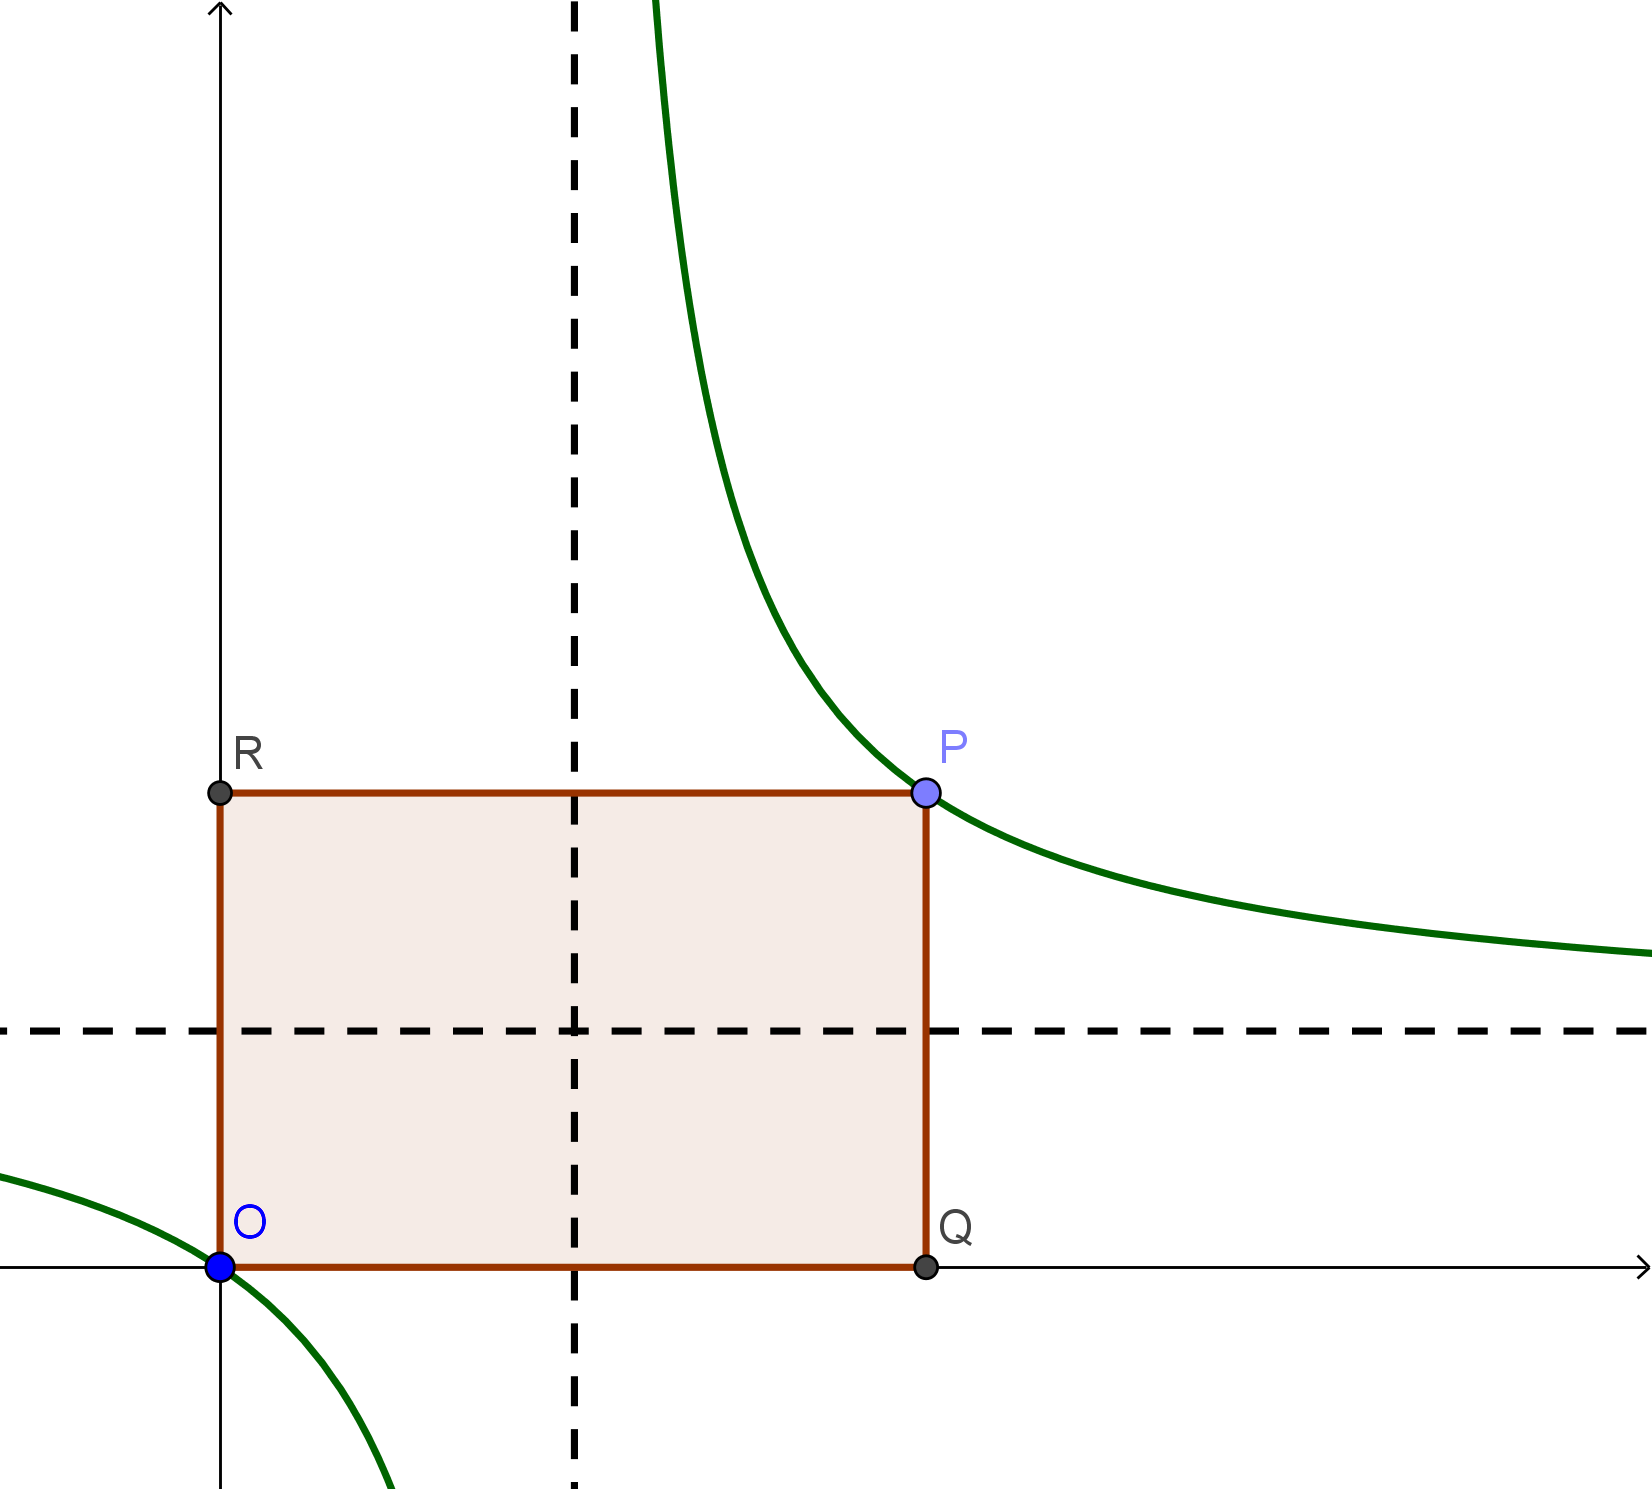
\includegraphics[width=0.9\textwidth]{1}
\end{center}

\(P=(a,b)\)라고 하면 \(\overline{PR}=a\), \(\overline{PQ}=b\)이고
\[b=\frac6{a-3}+2\]
이다.
(\(a>3\), \(b>2\))
그러면,
\begin{align*}
\square OQPR
&=ab\\
&=a\left(\frac6{a-3}+2\right)\\
&=\frac{6a}{a-3}+2a\\
&=\frac{6(a-3)+18}{a-3}+2a\\
&=6+\frac{18}{a-3}+2(a-3)+6\\
&=\frac{18}{a-3}+2(a-3)+12\\
&\ge2\sqrt{\frac{18}{a-3}\cdot2(a-3)}+12\\
&=12+12=24
\end{align*}
\end{minipage}
~
%%%
\begin{minipage}{0.45\textwidth}
방법 2)
\begin{center}
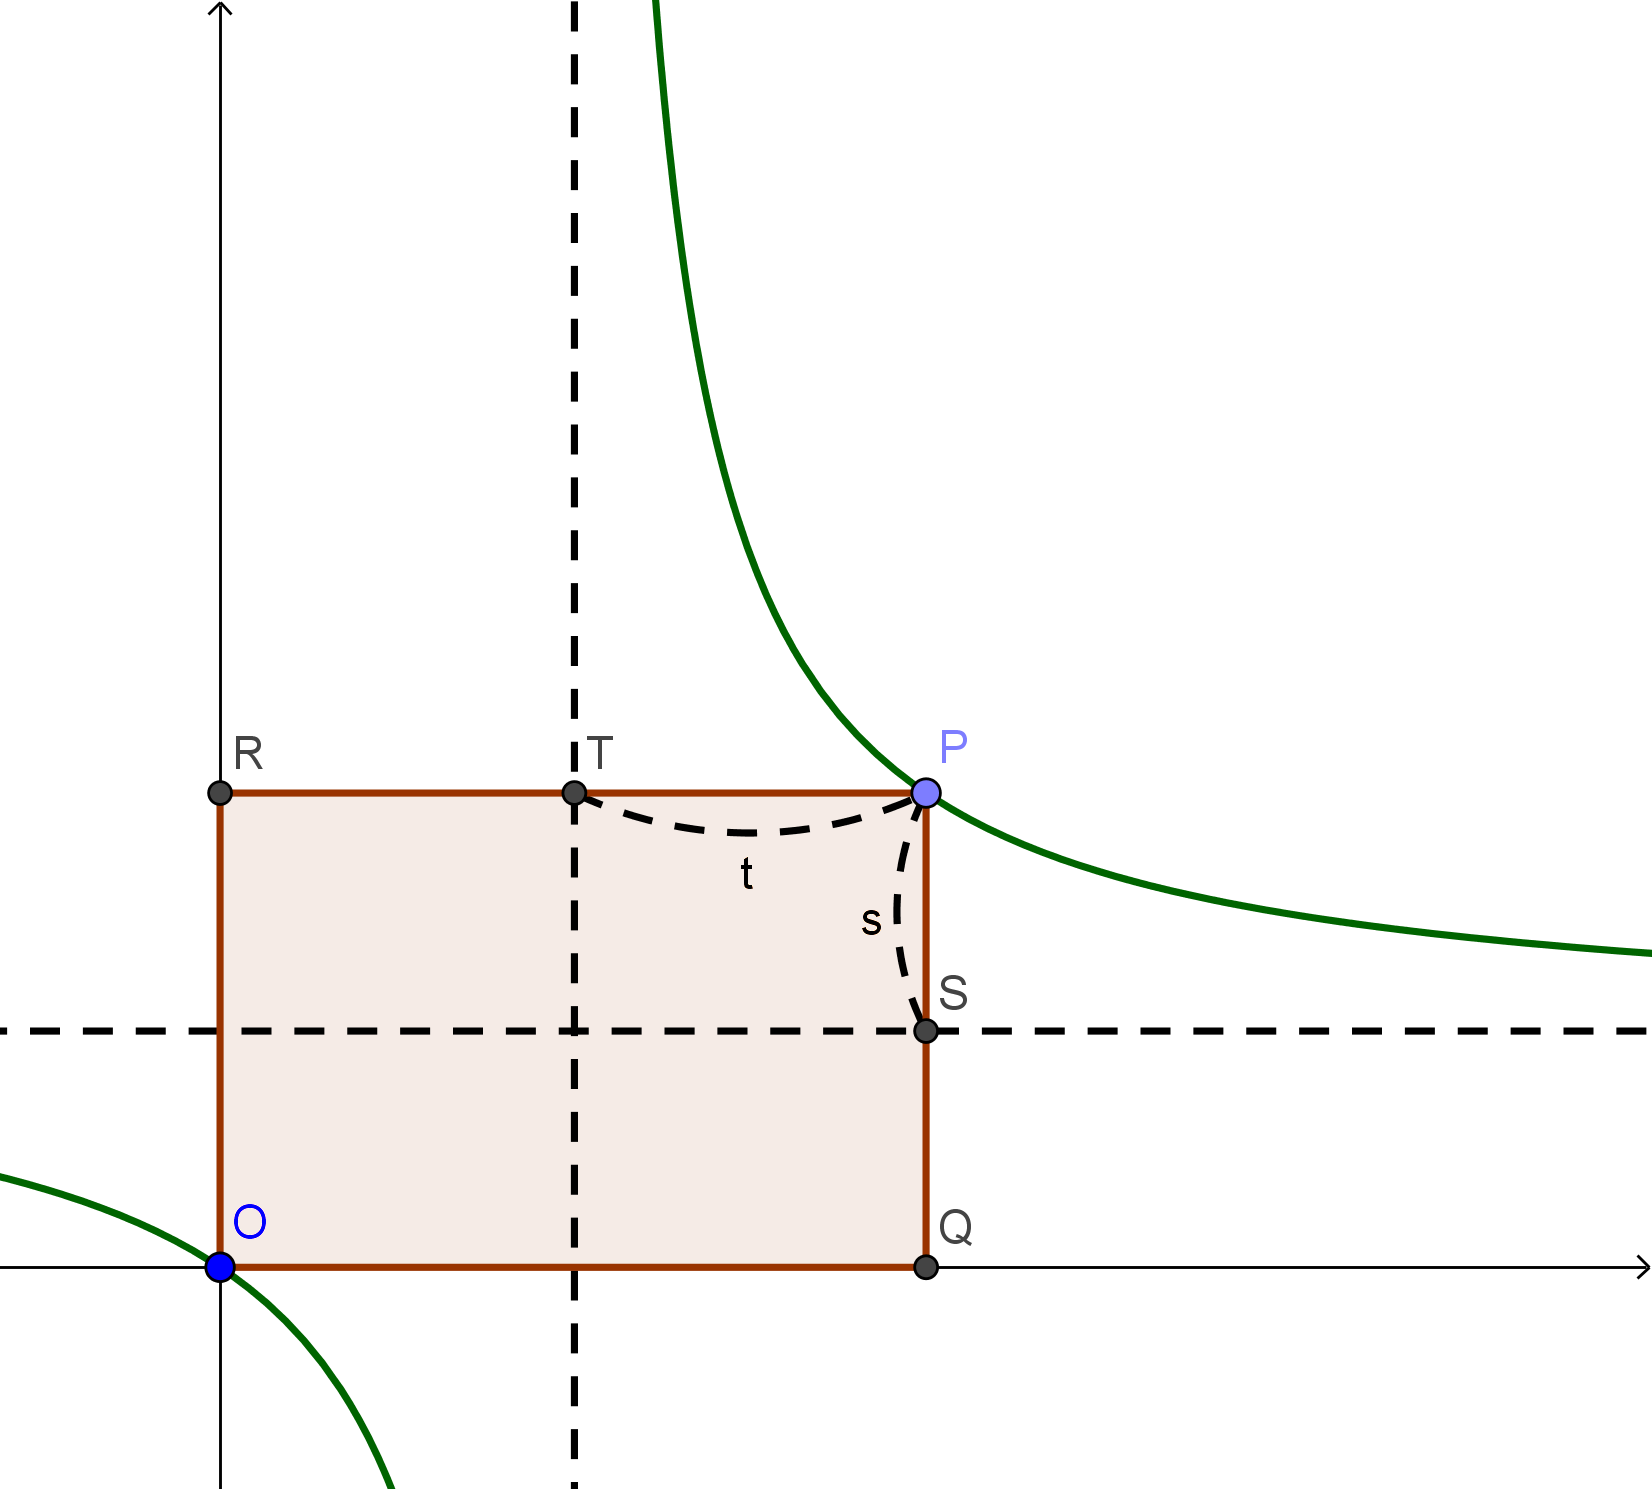
\includegraphics[width=0.9\textwidth]{2}
\end{center}

\(\overline{PT}=t\), \(\overline{PS}=s\)라고 하면 \(t>0\), \(s>0\)이고, \(P=(3+t,2+s)\)에서
\[ts=6.\]
그러면,
\begin{align*}
\square OQPR
&=(3+t)(2+s)\\
&=6+2t+3s+ts\\
&=6+2t+3s+6\\
&=12+2t+3s\\
&\ge12+2\sqrt{2t\cdot3s}\\
&=12+2\sqrt{6ts}\\
&=12+2\sqrt{36}\\
&=24
\end{align*}
\hspace{130pt}
\end{minipage}

\newpage
\begin{center}
\LARGE유리함수와 산술-기하 부등식
\end{center}

\bigskip
\begin{mdframed}[leftmargin=.2\textwidth,rightmargin=.2\textwidth]
\begin{spacing}{1.7}
유리함수 \(\displaystyle y=\frac8{x-2}+1\)의 그래프 점 \(P\)에 대하여, \(P\)에서 \(x\)축에 내린 수선의 발을 \(Q\), \(y\)축에 내린 수선의 발을 \(R\)이라고 할 때 직사각형 \(OQPR\)의 넓이의 최솟값을 구하여라.
(단 \(O\)는 원점이고 \(P\)는 제 1사분면 위에 있다.)
\end{spacing}
\vspace{0pt}
\end{mdframed}
\bigskip\bigskip

%
\begin{minipage}{0.45\textwidth}
\begin{mdframed}
방법 1)
\vspace{0.7\textheight}
\end{mdframed}
\end{minipage}
~
%%%
\begin{minipage}{0.45\textwidth}
\begin{mdframed}
방법 2)
\vspace{0.7\textheight}
\end{mdframed}
\end{minipage}


\end{document}